% As a sample.tex gernerate by uplatex				%請使用uplatex編譯
% uplatex mysample && ptex2pdf -l -u -ot "-kanji=utf8 " -od "-p B5"  mysample



\chapter*{大唐西域記序}
\setcounter{chapter}{15}

\hbox{}\hfill
尚書左僕射燕國公于志寧  

若夫玉豪流照,甘露灑於大千;金鏡揚輝,薰風被於有截。故知示現三界,粤稱天下之尊;光宅四表,式標域中之大。是以慧日淪影,象化之跡東歸;帝猷宏闡,大章之歩西極。

有慈恩道場三藏法師,諱玄奘,俗姓陳氏,其先潁川人也。帝軒提象,控華渚而開源;大舜賓門,基歴山而聳構。三恪昭於姬載,六奇光於漢祀。書奏而承朗月,遊道而聚德星。縱壑駢鱗,培鳳齊翼。世濟之美,欝為景胄。法師籍慶誕生,含和降德,結根深而䓲茂,導源浚而靈長。奇開之歳,霞軒日舉;聚沙之年,蘭薰桂馥。洎乎成立,藝殫墳素。九皐載響,五府交璧。以夫早悟真假,夙昭慈慧,鏡真筌而延佇,顧生涯而永息。而朱紱紫纓,誠有界之微網;寳車丹枕,寔出世之津途。由是擯落塵滓,言歸閑曠。令兄長捷法師,釋門之棟幹者也。擅龍象於身世,挺鶖鷺於當年。朝野挹其風猷,中外羨其聲彩。既而情深友愛,道睦天倫。法師勤服請益,分陰靡棄。業光上首,擢秀檀林;德契中庸,騰芬蘭室。杭策平道,苞九部而吞夢;鼓枻玄津,俯四韋而小魯。自兹遍遊談肆,載移涼燠。功既成矣,能亦畢矣。至於泰初日月,燭耀靈臺;子雲鞶悅,發揮神府。於是金文蹔啓,佇秋駕而雲趍;玉柄纔撝,披霧市而波属。若會斵輪之旨,猶知琴瑟之微。以瀉瓶之多聞,泛虛舟而獨遠。迺於轘轅之[地],先摧鍱腹之誇;井絡之鄕,遽表浮杯之異。遠迩宗挹,為之語曰:「昔聞荀氏八龍,今見陳門雙驥。」汝、頴多奇士,誠哉此言。

法師自幼迄長,遊心玄籍。名流先達,部執交馳,趍未忘本,摭華捐實,遂有南北異學,是非紛糺。永言於此,良用憮然。或恐傳譯踳駁,未能筌究,欲窮香象之文,將磬龍宮之目。以絕倫之德,属會昌之期,杖錫拂衣,第如遐境。於是背玄㶚而延望,指蔥山而矯迹。川陸綿長,備甞艱險。陋博望之非遠,嗤法顯之為局。遊踐之處,畢究方言,鐫求幽賾,妙窮津會。於是詞發雌黃,飛英天竺;文傳貝葉,聿歸振旦。太宗文皇帝金輪纂御,寳位居尊。載佇風徽,召見青蒲之上;迺睠通識,前膝黃屋之間。手詔綢繆,中使継路。俯摛睿思,乃製「三藏聖教序」,凡七百八十言。今上昔在春闈,裁「述聖記」,凡五百七十九言。啓玄妙之津,盡揄揚之旨。盖非道映鷄林,譽光鷲嶽,豈能緬降神藻,以旌時秀。奉 詔翻譯梵本,凡六百五十七部。具覽遐方異俗,絕壤殊風,土著之冝,人倫之序,正朔所曁,聲教所覃,著「大唐西域記」,勒成一十二卷。徧錄典奧,綜覈明審,立言不朽,其在兹焉。

\mycleardbpage
\setcounter{chapter}{15}
\chapter{賈元春才選鳳藻宮 秦鯨卿夭逝黃泉路}

\rubyfontsetup{\mgfamily\fontsize{8.5pt}{10}\selectfont}  % truely 7.760 pt in real dimen.

\par%
列位看官︰你道此書從何而来?\ruby[g]{說起根由雖近荒唐}{{\甲{自占地步。◯自首荒唐,妙!}}},細\ruby[Sg]{諳}{按}則深有趣味。待在下將此来歴註明,方使閱者了然不惑。
\par%
原来\ruby[g]{女媧氏煉石補天}{{\甲{補天濟世,勿認眞,用常言。}}}之時,於\ruby[g]{大荒山}{{\甲{荒唐也。}}}\ruby[g]{無稽崖}{{\甲{無稽也。}}}煉成高經\ruby[g]{十二𠀋}{{\甲{總應十二釵。}}},\ruby[g]{方經二十四}{{\甲{照應副十二釵。}}}𠀋頑石三萬六千五百零一\ruby[g]{磈。媧皇氏只用了三萬六千五百磈}{{\甲{合周天之數。}\蒙{◯數足,偏遺我。「不堪入選」句中透出心眼。}}},\ruby[g]{{只單單的剩了}}{{\甲{◯剩了這一塊便生出這}}}\ruby[g]{{一磈未用,便棄在此山青峺峰下。誰知此石自經煅煉之後,靈性已通,因}}{{\甲{許多故事。使當日雖不以此補天,就該去補地之坑陷,使地平坦,而不得有此一部鬼話。◯煅煉後性方通,甚哉!人生不能學也。}}}\ztxt{1A1}{\甲{妙!自謂落墮情根,故無補天之用。}}
見衆石倶得補天,獨自己無材不堪入選,遂自怨自嘆,日夜悲號慚愧。
\par%
一日,正當嗟悼之際,俄見一僧一道遠遠而来,生得骨格不凡,丰神迥{\ruby[gS]{别}{異},\戚{\warichu{這是眞像,非幻像也。}}說說笑笑%
\ztxt{1b1}{\teal{此下四百二十四字,戚本作︰「(說說笑笑來在峰下)席地而坐長談,見(一磈鮮明瑩潔的美玉,那僧托於掌上……)」\\\hfill%
(胡適)}}
\甲{\dahange{\CID{731}}}来至峰下,坐于石邉高談快論。先是說些雲山霧海神僲玄幻之事,後便說到紅塵中榮華富貴。此石聽了,不覺打動凡心,也想要到人間去享一享這榮華富貴;但\ruby[g]{自恨粗蠢,不得已,便口吐人言}{{\甲{竟有人問︰「口生於何處?」其無心肝,可笑可恨之極!}}},向那僧道說道︰「大師,弟\ruby[g]{子蠢物}{{\甲{豈敢豈敢。}}},不能見禮了。適聞二位談那人世間榮耀繁華,心切慕之。弟子質\ruby[g]{雖粗蠢}{{\甲{豈敢豈敢。}}},性却稍通;況見二師仙形道體,定非凡品,必有補天濟世之材,利物濟人之德。如蒙發一點慈心,擕帶弟子得入紅塵,在那富貴場中溫柔郷裡受享幾年,自當永佩洪恩,萬刼不忘也。」二仙師聽畢,齊憨笑道︰「善哉,善哉!那紅塵中有却有些樂事,但不能永遠依恃;況又有『美中不足,好事多魔』八箇字緊相連屬,瞬息間則又『樂極悲生,人非物換』,究竟是『\ruby[g]{到頭一夢,萬境歸空}{{\甲{四句乃一部之總綱。}}}』,倒不如不去的好。」這石凡心已熾,那裡聽得進這話去,乃復苦求再四。二仙知不可强制,乃嘆道︰「此亦『靜極思動,無中生有』之數也。旣如此,我們便擕你去受享受享,只是到不得意時,切莫後悔。」石道︰「自然,自然。」那僧又道︰「若說你性靈,却又如此質蠢,並更無奇貴之處。\ruby[g]{{如此也只好{{踮}}脚而已}}{{\甲{煅煉過尚與人{{踮}}脚,不學者又當如何?}}}。也罷,我如今大施佛法助你助,\ruby[g]{待刼終之日,復還本質,以了此案。你道}{{\甲{妙!佛法亦須償還,況世人之債乎?近之賴債者来看此句。所謂遊戲筆墨也。}}}好否?」石頭聽了,感謝不盡。那僧便念咒書符,\ruby[g]{大展幻術,}{{\甲{明點「幻」字。好! }}}將一磈大石登時變成一磈鮮明瑩潔的美玉,且又\ruby[g]{縮成扇墜大小的可佩可拿}{{\甲{奇詭險怪之文,有如髥蘇〈石鐘〉〈赤壁〉用幻處。}}}。\甲{\dahange{\CID{733}}}\dahange{〈甲戌〉}
\par%
那僧托於掌上,笑道︰「\ruby[g]{形體倒也是個寶物了!還只没有實在的好處,須}{{\甲{自愧之語。}\蒙{◯世上人原自據看得見處為憑。}\甲{◯妙極!今之金玉其外敗絮其中者,見此大不歡喜。}}}\ruby[g]{得再鐫上數字,使人一見便知是奇物方妙。}{{\甲{世上原宜假,不宜眞也。◯諺云︰「一日𧶠了三千假,三日𧶠不出一個眞。」信哉! }}}然後好擕你到那\ruby[g]{昌明隆盛}{{\甲{伏長安大都。}}}之邦,詩禮\ruby[g]{簪纓之族}{{\甲{伏榮國府。}}},\ruby[g]{花柳繁華}{{\甲{伏大觀園。}}}地,\ruby[g]{溫柔富貴郷去安身樂業。」石}{{\甲{伏紫芸軒。◯何不再添一句云「擇個絶世情痴作主人」?}}}頭聽了,\zmark{1A2}%
\ztxt{1A2}{\甲{昔子房後謁黃石公,惟見一石。子房當時恨不隨此石去。余亦恨不能隨此石而去也。聊供閱者一笑。}}
喜不能禁,\ruby[g]{乃問︰「不知賜了弟子那幾件奇處,又不}{{\甲{可知若果有奇貴之處,自己亦不知者。若自以奇貴而居,究竟是無眞奇貴之人。}}}知擕了弟子到何地方?望乞明示,使弟子不惑。」那僧笑道︰「你且莫問,日後自然明白的。」說着,便袖了這石,同那道人飄然而去,竟不知投奔何方何舍。
\par%
後来,又不知過了幾世幾刼,因有個空空道人訪道求仙,忽從這大荒山無稽崖青峺峰下經過,忽見一大磈石上字跡分明,編述歴歴。空空道人乃從頭一看,原来就是「\ruby[g]{無材補天,幻形}{{\甲{八字便是作者一生慚恨。}}}入世」,蒙茫茫大士,渺渺眞人擕入紅塵,歴盡離合悲歡炎涼世態的一段故事。後面又有一首偈云︰
\begin{quotation}
\par%
無材可去\ruby[g]{補蒼天}{{\甲{書之本旨。}}}%
\hspace{2zw}\ruby[g]{枉入紅塵若許年}{{\甲{慚愧之言,嗚咽如聞。}}}
\par%
此係身前身後事\hspace{2zw}倩誰記去作奇傳
\end{quotation}
\par%
詩後便是此石\ruby[Sg]{墮}{墜}落之郷,投胎之處,親自經歴的一段陳跡故事。其中家庭閨閣瑣事,以及閒情詩詞倒還全備,\ruby[g]{{或可適趣解悶,然朝代年紀,地輿邦}}{{\甲{「或」字謙得好。若用此套者,胸中必無好文字,手中斷無新筆墨。}}}國,却\truby[g]{反失落無考}{{\甲{據余說,却大有考證。}}}{{\蒙{妙在「無考」。}}}。空空道人遂向石頭說道︰「石兄,你這一段故事,據你自己說有些趣味,故編冩在此,意欲問世傳奇。據我看来,第一件,\ruby[g]{無朝代}{{\甲{先駁得妙。}}}年紀可考;第二件,並無\ruby[g]{大賢大忠、理朝廷治}{{\甲{將世人欲駁之腐言預先代人駁盡。妙!}}}風俗的善政,其中只不過几個異樣的女子,或情或痴,或小才微善,亦無班姑蔡女之德能。我縱抄去,恐世人不愛看呢。」

\par%
石頭笑答道︰「我師何太痴耶!若云無朝代可考,今我師竟假借漢唐等年紀添綴,\ruby[g]{又有何難}{{\甲{所以答得好。}}}?但我想,歴来野史,皆蹈一轍,莫如我這不借此套者,反倒新奇别緻,不過只取其事體情理罷了,又何必拘拘于朝代年紀哉!再者,市井俗人喜看理治之書者甚少而愛適趣閒文者特多。歴来野史,\ruby[g]{或訕謗君相}{{\甲{先批其大端。}}},或貶人妻女,姦淫兇惡,不可勝數。……




\chapter{畫圖測試}


\begin{minipage}<y>[htpb]{80mm}
	\begin{center}
    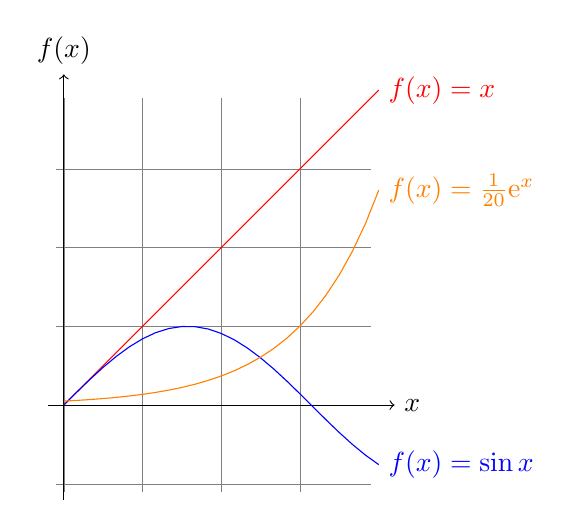
\begin{tikzpicture}[domain=0:4]
		  \draw[very thin,color=gray] (-0.1,-1.1) grid (3.9,3.9);
  		\draw[->] (-0.2,0) -- (4.2,0) node[right] {$x$};
		  \draw[->] (0,-1.2) -- (0,4.2) node[above] {$f(x)$};
		  \draw[color=red]    plot (\x,\x)             node[right] {$f(x) =x$};
  % \x r 表示弧度
		  \draw[color=blue]   plot (\x,{sin(\x r)})    node[right] {$f(x) = \sin x$};
		  \draw[color=orange] plot (\x,{0.05*exp(\x)}) node[right] {$f(x) = \frac{1}{20} \mathrm e^x$};
		\end{tikzpicture}
	\end{center}
\end{minipage}


\clearpage

\begin{minipage}<t>[htpb][80mm][t]{80mm}
	\begin{center}
		\vspace*{60mm}
    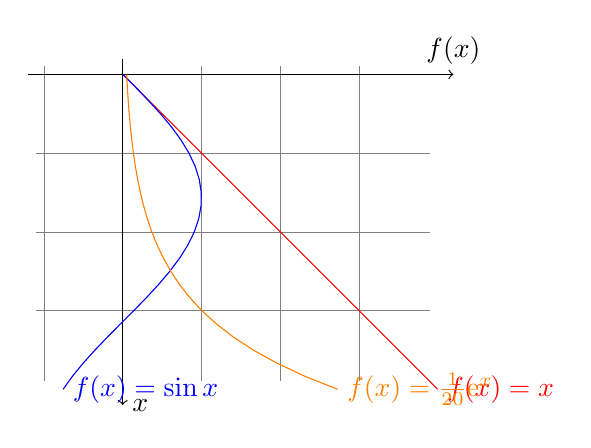
\begin{tikzpicture}[domain=0:4,scale=1,rotate=270]
		  \draw[very thin,color=gray] (-0.1,-1.1) grid (3.9,3.9);
  		\draw[->] (-0.2,0) -- (4.2,0) node[right] {$x$};
		  \draw[->] (0,-1.2) -- (0,4.2) node[above] {$f(x)$};
		  \draw[color=red]    plot (\x,\x)             node[right] {$f(x) =x$};
  % \x r 表示弧度
		  \draw[color=blue]   plot (\x,{sin(\x r)})    node[right] {$f(x) = \sin x$};
		  \draw[color=orange] plot (\x,{0.05*exp(\x)}) node[right] {$f(x) = \frac{1}{20} \mathrm e^x$};
		\end{tikzpicture}
	\end{center}
\end{minipage}

\chapter{公式測試}

\vskip 20 mm
\begin{minipage}<y>[htpb]{80mm}
		\vspace*{45mm}
	%\begin{center}
			{\normalsize With normalsize 10 pt in class (truely 9.13\,pt in real dimen):
				\[ \sampleEq \]\par}

			{\Large With Large 14 pt in class (truely 12.782\,pt in real dimen):
				\[ \sampleEq \]\par}

			{\footnotesize With footnotesize 8 pt in class (truely 7.304\,pt in real dimen):
				\[ \sampleEq \]\par}
	%\end{center}
\end{minipage}

\clearpage
\begin{minipage}<t>[htpb]{120mm}
		\vspace*{10mm}
	%\begin{center}
			{\normalsize 
				\[ \sampleEq \]\par}

			{\Large 
				\[ \sampleEq \]\par}

			{\footnotesize
				\[ \sampleEq \]\par}
	%\end{center}
\end{minipage}


\endinput